% !TEX TS-program = pdflatex
\documentclass[10pt,twocolumn]{article} 

% required packages for Oxy Comps style
\usepackage{oxycomps} % the main oxycomps style file
\usepackage{times} % use Times as the default font
\usepackage[style=numeric,sorting=nyt]{biblatex} % format the bibliography nicely 

\usepackage{amsfonts} % provides many math symbols/fonts
\usepackage{listings} % provides the lstlisting environment
\usepackage{amssymb} % provides many math symbols/fonts
\usepackage{graphicx} % allows insertion of grpahics
\usepackage{hyperref} % creates links within the page and to URLs
\usepackage{url} % formats URLs properly
\usepackage{verbatim} % provides the comment environment
\usepackage{xpatch} % used to patch \textcite
\usepackage{amsmath} % used for matrices

\graphicspath{ {./images/} }

\bibliography{refs.bib}
\DeclareNameAlias{default}{last-first}

\xpatchbibmacro{textcite}
  {\printnames{labelname}}
  {\printnames{labelname} (\printfield{year})}
  {}
  {}

\pdfinfo{
    /Title (YouTube Image Search: Is It Viable?)
    /Author (Christopher Linscott)
}

\title{YouTube Image Search: Is It Viable?}

\author{Christopher Linscott}
\affiliation{Occidental College}
\email{clinscott@oxy.edu}

\begin{document}

\maketitle

% Refer to rubic: https://docs.google.com/document/d/14caXj4RZ4pBAFtMEgXHtxMqi6gLjo8MnY1RSmGvkUgo/edit

\section{Problem Context}

What does the phrase "football coach" mean? What breed of dog is in this photo? Text-based search has been widely used since the 1990s \cite{WikipediaFullText}, but many issues have arised with it. While text is a fast, easy-to-use search tool, it's also imprecise and may require multiple search queries to find relevant information. Depending on where one is from, what dialect they use, words and phrases people use can have ambiguous meaning \cite{Beall2008}. In the worst case, if they cannot describe what they're searching for, getting information can feel paradoxical, as forming a search query given only visual context is difficult; you "don't know what you don't know." Difficulties in the ambiguity of language and the imprecise medium to describe what we're looking for, lead to more false positives, more time spent searching for the information within the results, and worst of all leads to more questions unanswered.

Current video recommendation methods, like YouTube, rely on textual information about the video using keywords \cite{Stanford2021}. Without knowing the name or a related keyword, one cannot simply search the web in hopes for an answer. Not only does image search help users tell the search engine what they’re looking for (with less ambiguity), but image-related search removes the need to annotate images online with keywords as image similarity can be used as a heuristic \cite{Adrakatti2016}.

Therefore, my solution emulates image search in YouTube, as a means to solve this information gap using related videos, while also offering times within videos where the relevant content is found. A user inserts an image of an object in real life or even a drawing (from their lecture notes for example), and my project returns videos with related images either from the thumbnail or the video frames. If related video frames are found within the video, times corresponding to these frames will additionally be returned.

By using images, there is far less ambiguity and taking a picture of something unknown is far easier than describing it. Therefore, my solution solves these problems of text-based search, and speeds up the searching process by including relevant times within videos, so users don't always have to sift through videos for relevant information.

\section{Technical Background} 

YouTube videos can be broken down into images through both the thumbnail, an image preview of the video content, and the individual frames which make up the same video. Determining a description of an image means taking into account the positions of objects, edges, shapes, and other characteristics of objects that may render useful. Mathematical "descriptions" of images are created, containing numerical information of visual characteristics (called features), which can be compared to each other using distance-based or object-based methods. Upon the insertion of a query image, a description of the query image will be computed and will be compared against stored descriptions of other images (whether frames or thumbnails) to determine related videos.

Creating these "descriptions" of images required using a Convolutional Neural Network (CNN), a specialized Artifical Neural Network (ANN) designed for pattern recognition. A more semantic description relating to the objects in the image, was created utilizing a Faster-RCNN (RCNN), or Region-based Convolutional Neural Network. The description of these images will look like vectors and maps respectively, the CNN vectors containing number which represent the "activation" or how much particular features (such as shape, texture, or color) exists within different regions of a given image. The RCNN will return JSON, or a map which for every object class it sees ("dog"), tells the number of those objects it sees in the image.

Upon inserting an image, finding relevant information means finding images (that refer back to a given video) which relate to our input image by comparing these features. By utilizing video frames in addition to the thumbnails, we can determine the time within the video which is relevant, from the number of frame, as we grab one frame every second.

With a Convolutional Neural Network, we have 3 important layers which are the Convolutional Layer, Pooling Layer, and Activation Layer. While the Fully Connected Network is important in most neural networks, as we want the low-level image representation and not the high-level object classification the model makes, we remove this layer. Convolution refers to the combination of two functions; in the case of our CNN, the convolution combines the input information (in the form of raw pixel values) with the values of a sliding filter, merging them together. The convolution is performed through a non-full connection of the neurons unlike the ANNs, meaning the neurons in the next layer only get inputs from corresponding portions of the previous layer \cite{Albawi2017}. In a sense, the neural network will now look at local regions of the picture.

Suppose we have a matrix F of raw pixels and our filter matrix G. To compute the convolution or merge the raw pixels and filter matrix G together, we compute the convolution of two matrices which is simply the sum of the products of the overlapping grid squares \cite{Dumoulin2018}:

$$ \begin{pmatrix} a & b \\ c & d \end{pmatrix} * \begin{pmatrix} e & f \\ g & h \end{pmatrix} = \begin{pmatrix} ae + bf + cg + dh \end{pmatrix} $$ 

So, if we had a large image, we would compute many of these summed products, resulting in a large matrix of the convolved matrices of image pixels and filter (which stays the same). Depending on parameters of stride, kernel size, and padding around the image, we get a output (called the feature map) which represents the merging of the image and filter. The filters that we choose, or are pre-trained normally, will affect the image in different ways in order to highlight different characteristics of the image when we perform these convolutions in the Convolutional Layer. This becomes important, depending on the filter we choose. For example, the Sobel Filter \cite{Bogdan2019} acts as a edge detector, where different values in the matrix can detect different edges. So, when our image is passed through this layer, it essentially highlights the edges of the image, which I'll describe as positive "activations" of that feature being an edge. With these activations of these features, the CNN can learn information such as edges, textures, colors, and other characteristics and combine them to make decisions on what characteristics it sees of specific regions. Overtime, through passing these features further into convolutional layers, the model can take lower-level features (such as edges or textures) and begin to combine and get activations of higher-level features (such as noses, heads, and eyes) until it has a very semantic representation of the image.

The unsung hero of the CNN is the pooling layer. The pooling layer acts as a feature "summarizer", where it grabs the maximum or average value of a group (2x2, 3x3) of grid squares (or pixels) and uses this as one grid square of the output. In a similar fashion to the kernel in the convolutional layer, the pooling layer will be simply "slide" over the image and compute the maximum of the activations of features it sees. There are several things this layer does: it reduces the size of the input overtime (reducing the complexity for deeper layers) \cite{Albawi2017}, reduces the output to something more readable (highlighting where and how much a feature is present), reduces the overall computation (since with our deeper levels, we only look at these summarized activations as opposed to the entire image), and it can tells us spatial information which which helps the model perform well in conditions where the image is translated (moved side to side) or rotated as the positions of features will change (but the activations will not). As well as, in the context of an image, the pixels and features/characteristics nearby each other are normally related.

\begin{figure}[h]
  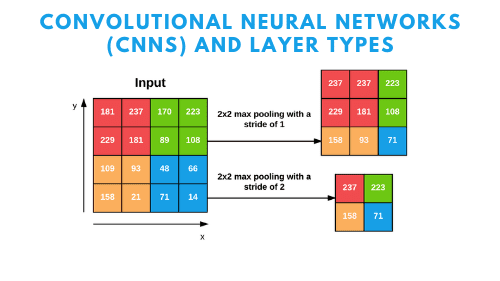
\includegraphics[width=8cm]{max_pooling.png}
  \caption{A diagram of 2 by 2 max pooling on a 4 by 4 matrix where the window slides over either one or two grid squares (stride of 1 or 2) after every pool.}
  \centering
\end{figure}

Finally, we have the activation layer. Depending on the choice of activitation, the model will either highlight the maxima and/or minima. As many models have had success with the ReLU activation layer (due to faster learing speeds) \cite{Ide2017}, it is the favorite and the Xception model includes this activitation function as well. It will alter the values of the outputs of the convolutional and pooling layers, by either storing a value of 0 or the value (if the value is higher than 0). The activation layer essentially captures what features exists, as opposed to unnecessary information (such as where features don't exist). By doing so, we summarize the image features further for the next layer, reducing the complexity.

\begin{figure}[h]
  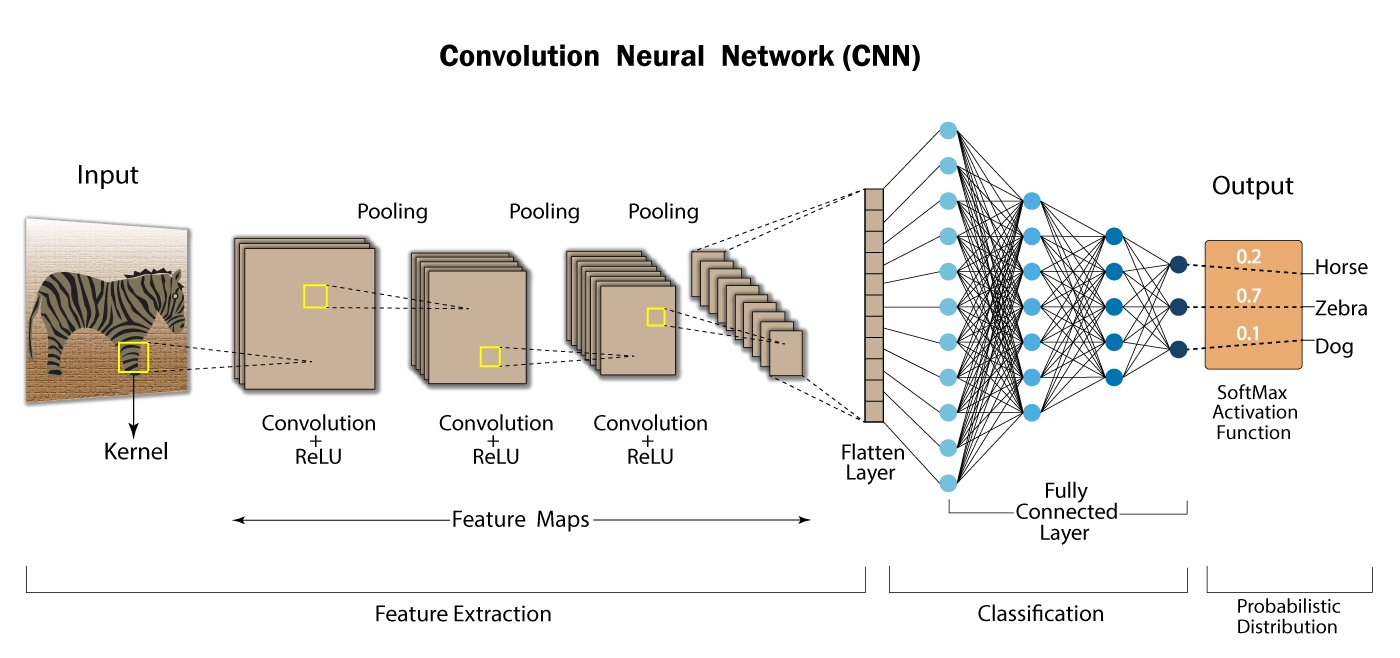
\includegraphics[width=8cm]{cnnlayer.jpg}
  \caption{A diagram of all the layers in a Convolutional Neural Network. \cite{Swapna2020}}
  \centering
\end{figure}

While the Convolutional Neural Network is an excellent model in deriving features from an image, one problem is that it sees the image is one way. The pooling layers of the Convolutional Neural Network will group the activiations of features using one size of square grid, i.e. it looks at the characteristics of the image through one size of window. However, to look at the image in different ways, an algorithm known as RMAC (Regional Maximal Activations of Convolutions) can be implemented on top of the CNN to look at the activiations of features (i.e. the feature maps) through many lens (i.e. sizes of square grid). Instead of computing the description through one "lens", we compute many different vectors based on different sized regions (to grab small and big characteristics/objects of the image) and combine them to form a vector which captures many different perspectives. Not only is this just as efficient as the normal CNN (as we just use the feature maps from the neural network), but this algorithm has proven to perform better than normal standard CNNs in image classification \cite{Tolias2016}.

Moving on, the Faster R-CNN is a third-generation object detection model, sprouting from the original R-CNN. The Faster R-CNN utilizes a Region Proposal Network (RPN) and convolutional layers (as discussed above) to determine the objects present. A Region Proposal Network will take any size image as input and determine how strongly it believes rectangular regions may have/be an object, by giving them an "objectness score" \cite{Ren2016}. To generate the proposals (of where objects may be), a small neural network is slid across the feature maps of the image (of the final convolutional layer) to generate a objectness score for regions of the image. Once it has determined regions (by having a threshold objectness score and activation function), these regions (of the feature map) will be fed into a fully-connected layer, which will determine the object within the region \cite{Ren2016}. Applying this to all the regions of the image, we can determine all the objects (with sizes, bounding boxes), where the objects are present in the photo.

To compute the "distance" or the similarity between two images, we compute the distance between the image representations (which are high-dimensional vectors). The distance metric used is Euclidean distance, which computes the distance between two image vectors $V_1$ and $V_2$ of dimension $d$ by computing the squared difference between the two vectors: $$D(V_1, V_2) = \sqrt{\sum_{i=0}^{d} (V_{1i} - V_{2i})^2}$$
$$ = \sqrt{(V_{11} - V_{21})^2 + (V_{12} - V_{22})^2 + ... + (V_{1d} - V_{2d})^2 }$$ where $V_{1i}$ and $V_{2i}$ are the values of the image vectors in the $i$th dimension. For the Object Detection Model, we used our own implementation (for ease-of-use and simplicity), which calculated the score based on the number of matching object classes and the difference in the number of objects (per matching class). To summarize, to get a score based on objects, we calculate a score based on (per matching object class) the sum of all the confidence scores (from the database image) multiplied by the reciprocal of the difference in the number of objects in the two images. To compute the score based on objects: $$OS(I_1, I_2) = \sum_{i = 0}^{c} \frac{1}{|I_{1i} - I_{2i}| + 1} \cdot (\sum_{all \ objects \ in \ I_{2}} o_s)$$

where $I_{1i}$, $I_{2i}$ are the number of objects for a given object class $i$ (up to the $c$ classes they share), $o_s$ is an individual object confidence score. 

\section{Prior Work}

Many image-related applications have been developed around solving the information/curiosity gap. A popular application is Google Lens, an application which in real time can analyze an image (whether it has text or a given object) and identify the object or text. Furthermore, image-related search applications, such as Google’s reverse image search, are very useful in determining the source of an image or determining similar images based on an input image. In fact, it’s being used often for educational purposes such as with plant identification \cite{Moore2018}. In a similar way to how Google Lens and Google’s reverse image search aims to solve the information gap (given only visual context), my application serves to solve it using related videos as opposed to a purely trained AI model on the classification of objects.

To go on, researchers at Stanford have utilized video frames within a given video (along with labeled good and bad thumbnails) to train a convolutional neural network to determine what frames of that video would constitute as a good “thumbnail”, or image preview to capture a user’s attention \cite{Stanford2017}. Extending this idea, we utilize the video frames in order to gather images to act as “markers” for the videos; when an user-given image matches, it references the video and/or the time within it.

Along with classifying YouTube thumbnails together, neural networks have also proven to be able to learn to cluster YouTube thumbnails together, categorizing them into different categories without the help of tags (i.e. labeled categories on the videos). Utilizing k-means clustering, they were able to compare and determine that a clustering algorithm could categorize videos by their thumbnails as well as YouTube did manually with tags \cite{Stanford2021}. As my dataset is labeled by category and neural networks have shown to categorize based on features as well, likewise I could extend this idea to segment images and develop the clusters/categories in an unsupervised manner with a similar combination of neural networks (CNN) and finetuning to increase the accuracy of my search tool.

As another possibility for this project, Noa Garcia and George Vogiatizs use a Convolutional Neural Network to create spatial-temporal visual embeddings, which compress the the visual information on videos into a global vector, extracting the meaningful visual information from static images. The models learns, through labeled training data, how to project them to a common embedding space where they're easily compared \cite{Garcia2018}. With this method, they were able to outperform many state-of-the-art systems, having a higher speed and accuracy as compared to other methods such as pre-trained CNNs. While my work primarily utilizes a pre-trained CNN (as my data is unlabeled), if there was access to labeled data, this could be a next step for this project. As well as, in a similar way to Inverted Indexing or clustering, we can construct a common space (or mapping from keywords to images) to fetch related videos as opposed to common distance metrics across all images which can be slow.

\section {Methods}

While videos from other platforms such as Dailymotion, Vimeo, or Twitch could've been utilized, as the YouTube video platform has many videos in different categories, YouTube's diversity of videos is useful for creating a database to query from which can have relevant videos for many different query images presented to it. Therefore, as datasets never included raw videos to download directly from, I fetched from the Google's YouTube8M Dataset, with the intention of grabbing the YouTube IDs (ids map to an unique video) and using them to download the videos directly on to my hard drive. The dataset returned data in the form of tensorflow record files (*.tfrecord), which contained high-level features of the video (such as cateogry and a general description), and a fake id related to the YouTube video. So, using \href{https://www.tensorflow.org/api_docs/python/tf/io}{tensorflow's parser}, I parsed the tensorflow record files, obtaining the fake id assigned to a video. With the fake id, I could grab the real YouTube ID assigned to the video through \href{https://research.google.com/youtube8m/video_id_conversion.html}{instructions provided by Google}, and download the video and thumbnail by using a python module called yt-dlp. As grabbing the YouTube ID and corresponding YouTube video/thumbnail took large amounts of time, I asynchrously fetched the YouTube IDs and upon arrival (or the completion of the HTTP request), I used multithreadding to concurrently run the downloads of the YouTube videos and thumbnails. To get the frames from the youtube videos, useful bash scripts provided by \href{https://github.com/gsssrao/youtube-8m-videos-frames}{gsssrao}to use the ffmpeg library to grab the frames of each video, name them (so if we query a frame, we can link back to the video), and store them in a seperate directory.

After obtaining the thumbnail and the corresponding video frames, I used a python library called opencv2, to load the images as a manipulatable 5D array of the image's pixels, with a size of the image's width, height, and number of channels (3 for red, green, and blue values of a pixel). To match the input expected by the models, these image arrays were resized to have a width and height of 299 pixels each. As YouTube thumbnails and frames are unlabeled images, with real-life objects present within them, I utilized the Convolutional Neural Network (CNN) which can learn and describe characteristics of objects and regions of images. To avoid training the Convolutional Neural Network (as I cannot train the neural network with unlabeled images), I utilized a pre-trained model, one trained with images from ImageNet of many different objects, so the training wouldn't be conducted by myself (which would require labeled data and time to train). Therefore, the CNN learns to detect and describe characteristics such as colors, shapes, and textures of real-life objects (which people are likely to query with). As a final desire, as efficiency becomes important when computing millions of images to decrease the amount of computing power and time for the image. With this characteristics in mind, the Xception model was a clear choice, as the model was extremely efficient, and it has a high top-five accuracy for image classification \cite{Chollet2017}, which is important in the context of related videos (where finding many good options can be better than finding only one great option) \cite{Stancic2022}. 

With CNN Models, in its normal state, there are two parts: the feature (characteristic extractor) extraction and classification portion (using fully connected layers). The output of the classification (from the fully connected layer) is far too semantic and researchers found that removing the fully connected layers of the model improved the accuracy and ability to compare images based on similarity \cite{Qian2020}. Therefore, to construct the AlteredXception (as named in the code), the Xception model was first created, and using the keras model, I removed the final fully connected layers of the Xception model, and made the final output the Pooling Layer. By having the final output being the Pooling Layer, the final output will consist of the flattened feature maps which tells us the high-level characteristics of regions of the image.

While the AlteredXception model is an excellent model in deriving features from an image, one problem is that it sees the image is one way. The pooling layers of the Convolutional Neural Network will group the activiations of features using one size of square grid, i.e. it looks at the characteristics of the image through one size of window. However, to look at the image in different ways, an algorithm known as RMAC (Regional Maximal Activations of Convolutions) can be implemented on top of the CNN to look at the activiations of features through many lens (i.e. sizes of square grid). Instead of computing the description through one "lens", we compute many different vectors based on different sized regions (to grab small and big characteristics/objects of the image) and combine them to form a vector which captures many different perspectives. Not only is this just as efficient as the normal CNN (as we just use the feature maps from the neural network), but this algorithm has proven to perform better than normal standard CNNs in image classification \cite{Tolias2016}. In the search to find a worthwhile image representation/description, testing the normal CNN versus this adaption can help determine if the added algorithm improves the results. To distinguish this adapation of the CNN from the normal CNN, I will refer to this adapation as the RMAC model. To build the RMAC model, utilizing code from Gordo \cite{Gordo2016} (readapted from Tolias \cite{Tolias2016}) and my implementation of the CNN, I combined them together.

In combination with the AlteredXception and RMAC model, a pre-trained Object Detection Model, called the Faster R-CNN model, was utilized for its accuracy and ease-of-use with general object classes. While it couldn't pick up on nuances very well, it can be used as a discriminator as well as for grabbing relevant (but not specific) videos very easily. To implement this model, the gluoncv library was utilized, which had a pre-trained version of the Faster R-CNN. After implementing and configuring these models, I began using the models to gather predictions/descriptions of various images from frames and thumbnails I gathered, passing them through the model and storing them away.

To store these image descriptions, my file system was used as a database, consisting of only JSON and NPY files. JSON files were initially used as they allowed me to maintain order and also check for duplicate predictions in my database. By storing the image paths as a key and the predictions as a value, I can simply check if an image path already exists within my JSON before computing the prediction (and wasting time creating duplicate predictions). As well as, I can use it to order my image paths and view it relatively easily. However, a big problem with JSON files is that loading the files take a long time, which in the context of an user interface and computing other predictions, can mean long wait times (on the magnitude of minutes) to load and have the prediction maps ready to be queried from or added to. So, as numpy files store and load numpy arrays much more efficiently compared to JSON files \cite{StackOverflow2016} and the overall ease-of-use with the numpy library (as my image representations were large numpy arrays), .npy files were used to store the image representations. To maintain the benefits of JSON with duplicates, I created a .npy file for the image representations (essentially a giant array of numpy arrays), and a JSON file which mapped an image path to the index of where the corresponding image representation is within the numpy array. So, the numpy files are faster to load and store, are smaller in size (as numpy has methods to efficiently store their arrays in npy files), and we still gain the benefits of JSON previously stated. For the Object Detection Model (unlike the other models), inverted indexing could be utilized for faster querying. Inverted Indexing is the process of mapping "words" to image as a way to determine and find more related images quickly. If our query image has visual words computed, we can use them to find other related images based on matching object classes. In the case of the Faster-R-CNN model, images had representations consisting of the objects' classes, sizes, and the model's confidence scores. Therefore, we can use inverted indexing to store an object class and map it to image paths which had the same object class. Each image path would also map to its confidence score of that object classes, so when we query, we can favor images where the model was more confident. By using this style of "database", when we compute the objects of an image, we can use the objects we find to query for images (and therefore videos) with related objects very quickly (since we don't look at all images, only those which match).

After attaining the descriptions of our YouTube images through these models and storing them away, the description of the query image will be computed using the same methods. To compare the descriptions created by the CNNs, I utilized Euclidean distance, or the sqaure root of the sum of the squared differences between the vectors. With this distance, we are essentially computing the difference of features within regions of the image. If there are more regions with different characteristics between images, they are viewed as farther in distance. If regions has similar characteristics in many regions, they were viewed as closer together. For descriptions created by the Object Detection Model, I computed a score (shown in Technical Background) based on the number of matching object classes and the difference between the number of objects (per class) in the query image and the number of objects in the database image. With similar images, they should have the same number of matching objects (images with two dogs should return images with two dogs). As well as, the number of matching classes matter (images with a dog and bike should return images with a dog and bike and not just dogs or bikes). By computing these differences, we return the relevant videos based on a high object score or a low Euclidean distance. 

% \begin{figure}[h]
%   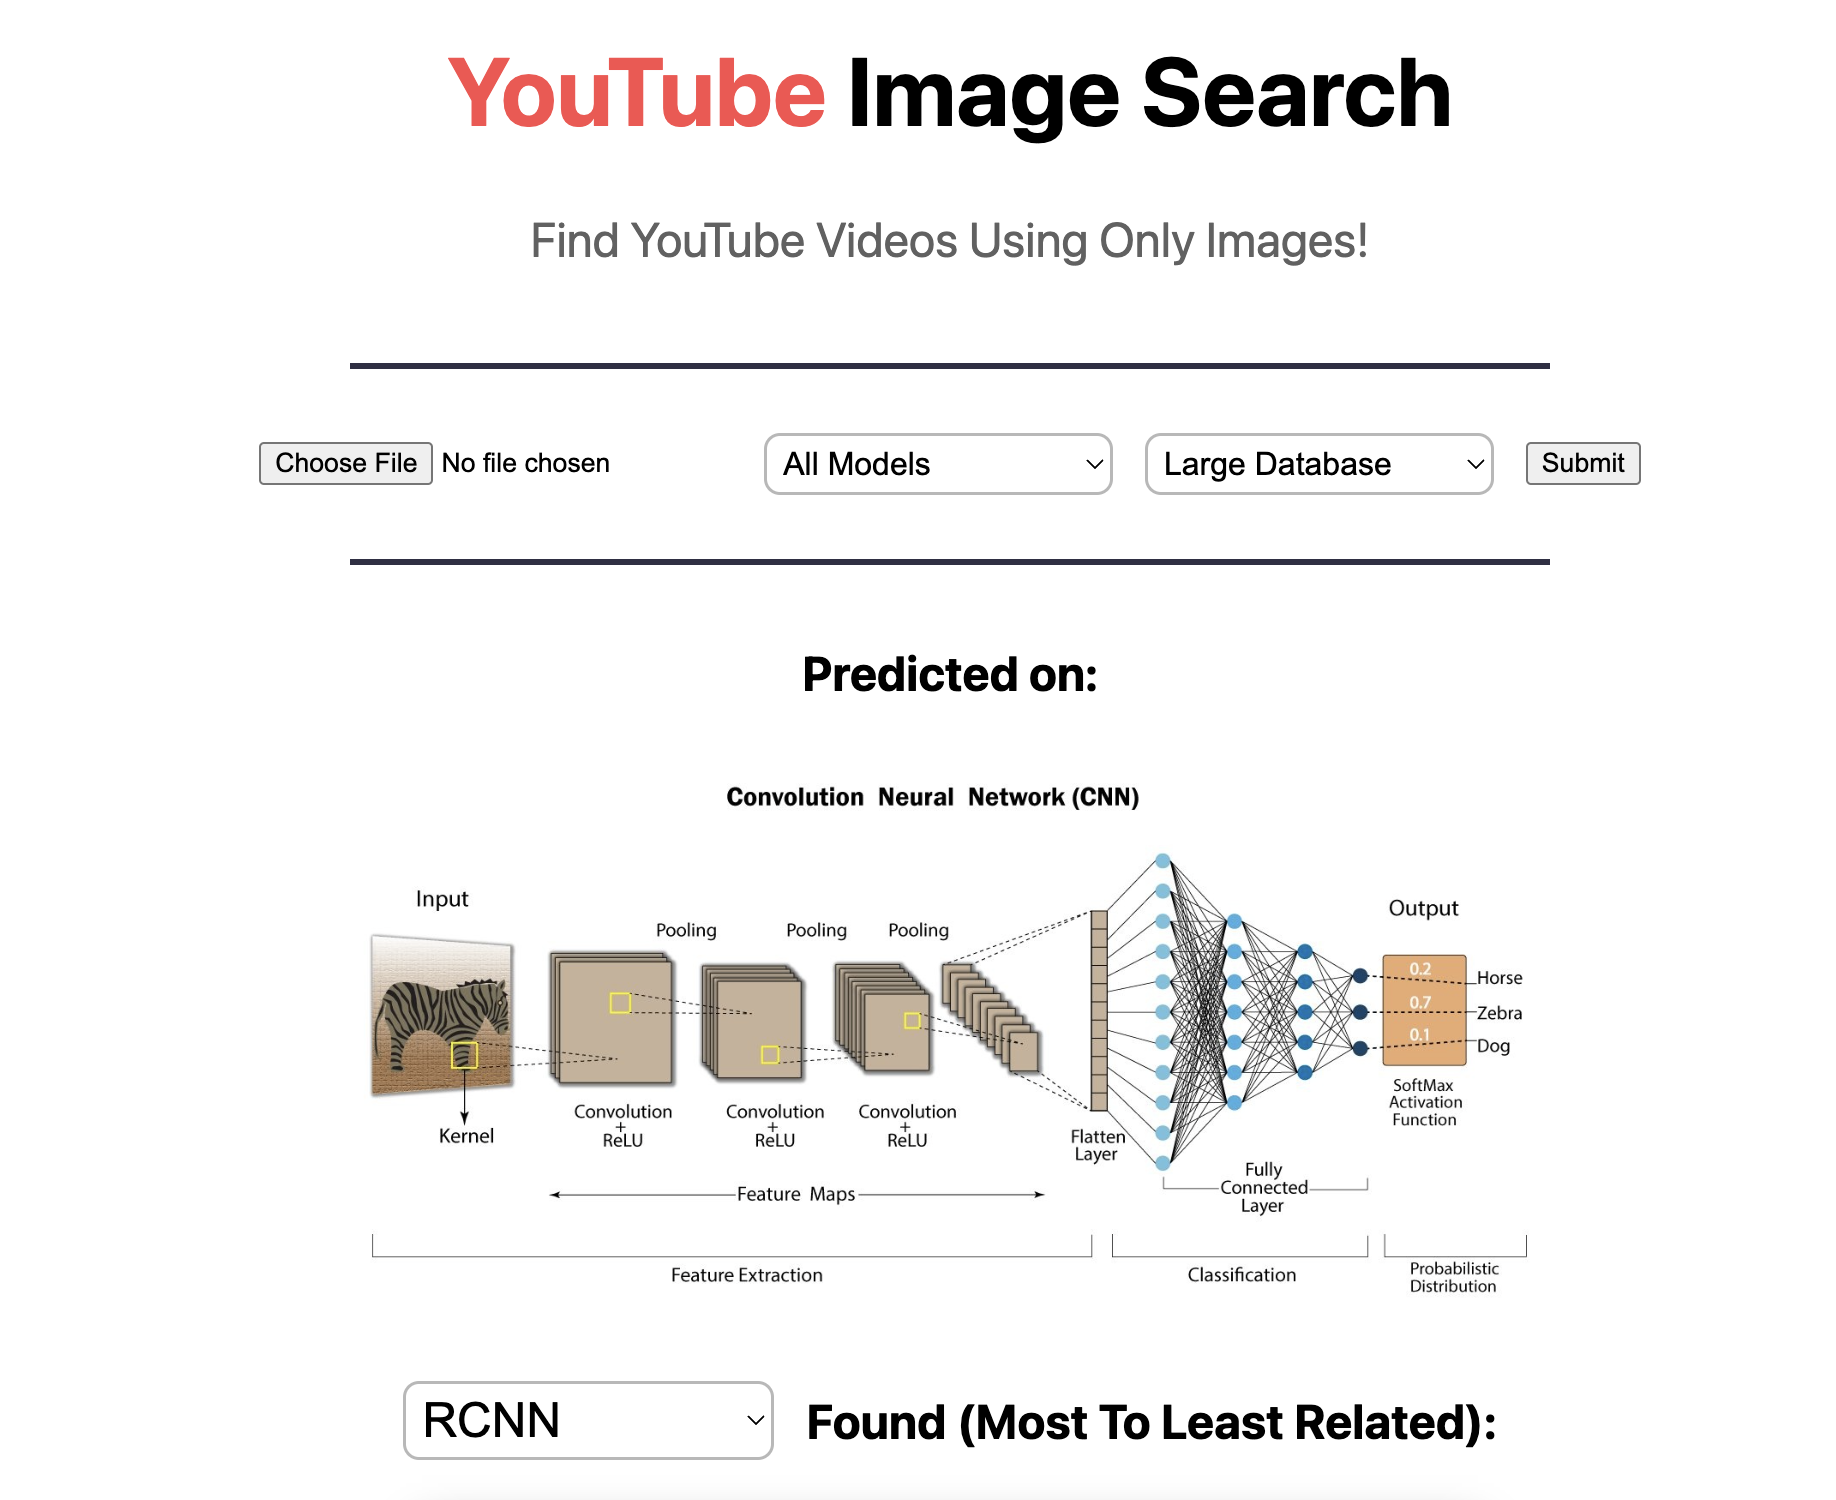
\includegraphics[width=8cm]{ui_form.png}
%   \caption{The user interface to submit query images.}
%   \centering
% \end{figure}


With the comparison in place, we have a way to get related videos from the query video. To make this search tool, I utilized flask, a Python library, which can quickly make a web server to serve HTML, CSS, and JS files to show the relevant videos and provide an input to take in query images. Utilizing HTML and CSS, I created a simple, easy-to-use website which would take the query image and send a POST request to my web server with the image. With the query image from the user, I would compute the image description and relevant videos (based on the models' predictions) and return the relevant videos for each model in the form of JSON. Utilizing Javascript, I parsed my model data and created sections to store each individual video (with iframes) and individual times (which became clickable buttons to go to that time of the video) for each video. Not only does this user interface showcase the accuracy and performance of the models and database, but it provides a preview into the benefits of image search through an interactable interface.

% \begin{figure}[h]
%   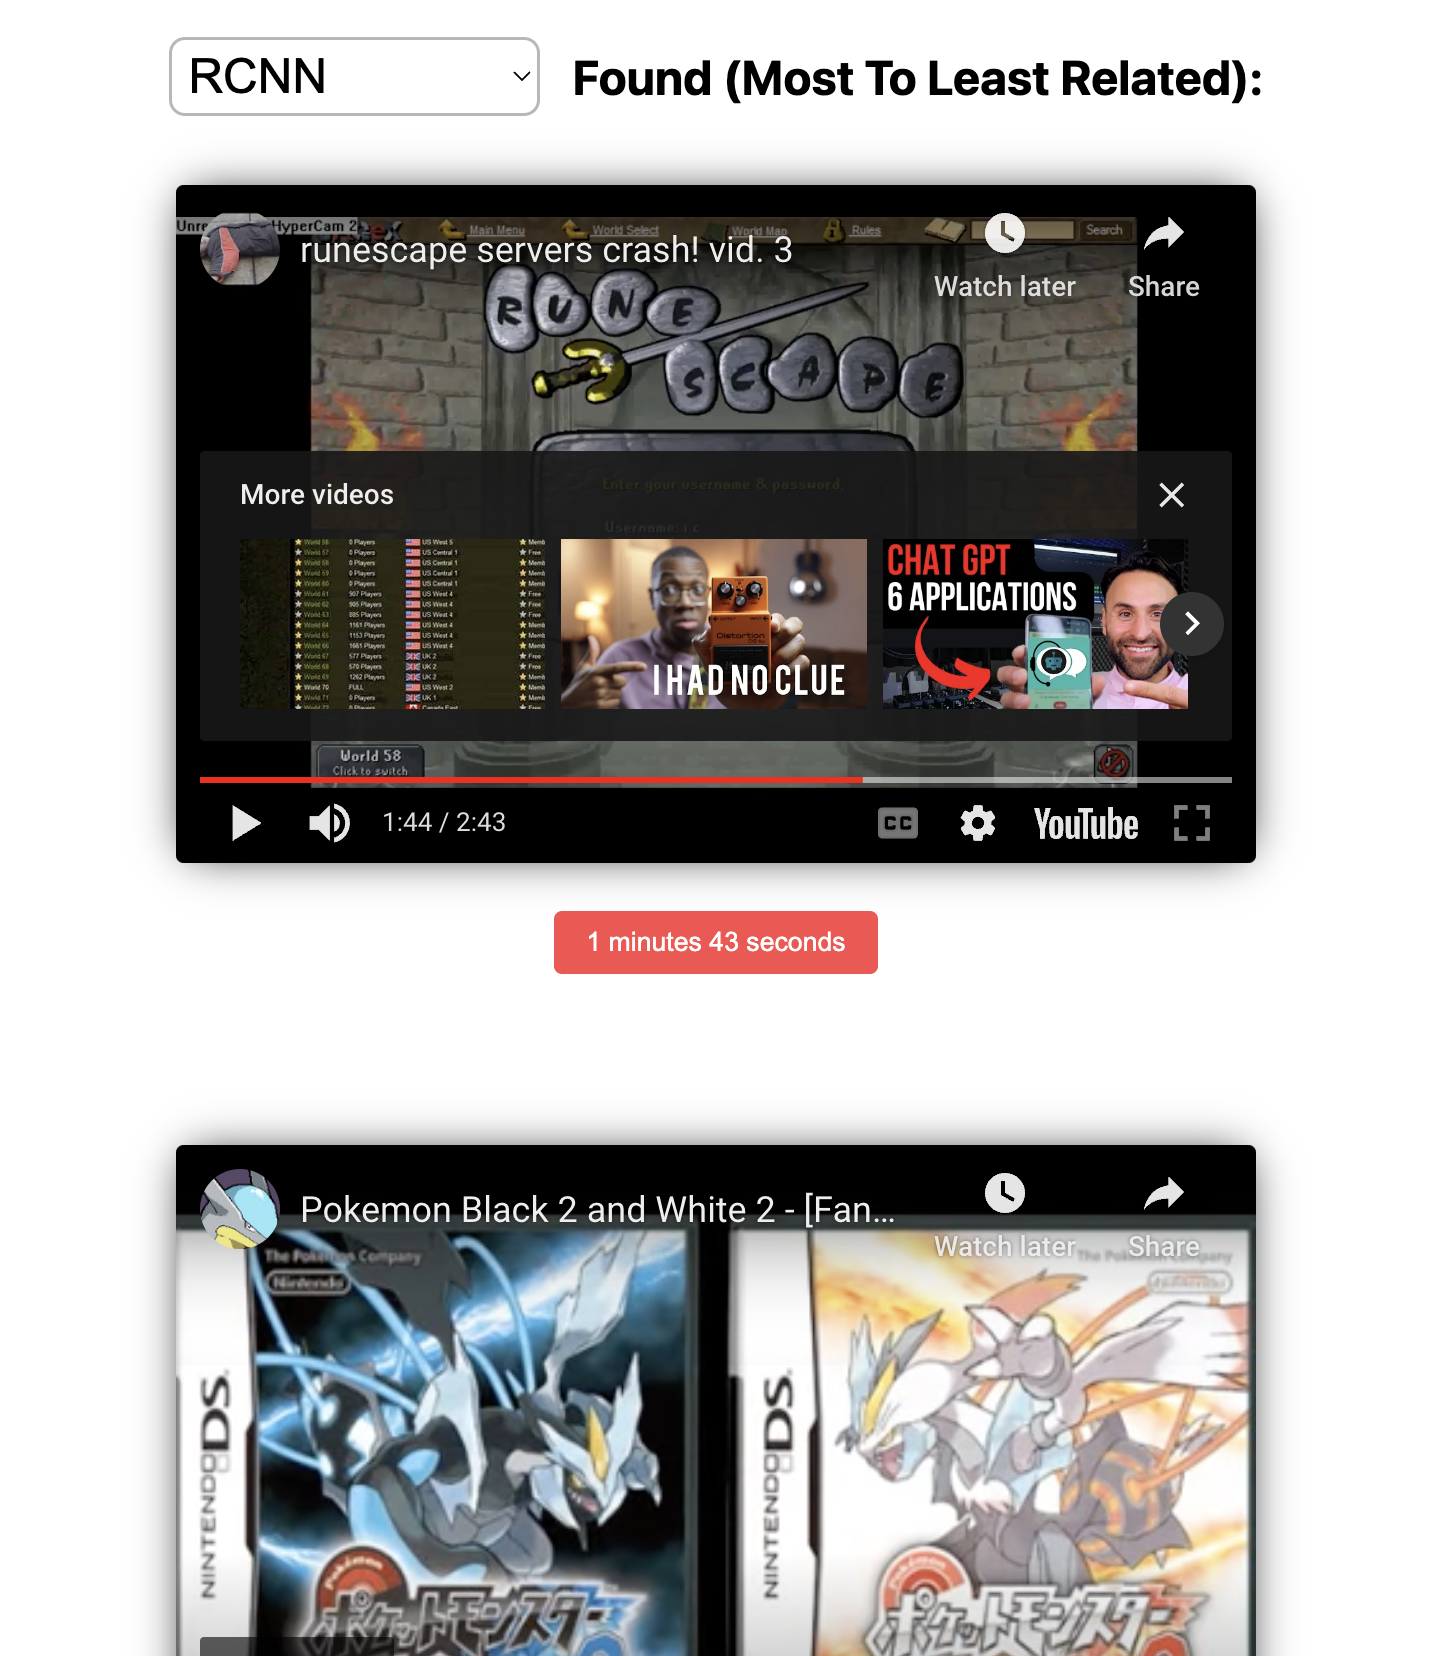
\includegraphics[width=8cm]{ui_predictions.png}
%   \caption{The interface for showing related videos.}
%   \centering
% \end{figure}

\section{Evaluation Metrics}

While creating this image search tool, there were three questions asked: the model's ability to find specific, relevant videos (such as a golden retriever versus a english bulldog), the model's performance under conditions of image manipulation, and most important how the model would perform under a small or large number of videos (with diverse or very related videos).

To evaluate this image search tool, I utilized variants of a query image and reported the difference between my predictions and the models' predictions of the most relevant videos. To begin with, an important and overarching metric is similarity and the ability to pick up nuances and return specific items, either in the context of a small or large number of possibilities. As an example, if we submit an image of a golden retriever into a dog database, we should expect the model to return golden retriever videos, and not just any dog videos.

Therefore, with dog, game, and art videos, I downloaded one hundred random videos from YouTube8M's dataset of that corresponding category, downloading the frames and thumbnails as well. As content-based image retrieval doesn't have a common method of obtaining "relevant judgements" for a query \cite{Muller2001}, I determined, with my own judgement, descriptions of these videos and a suitable query image that had many possible relevant videos. With this query image, the ground truth, or the top ten most relevant videos, was picked based on the same judgement. After having the models compute the image representations of the frames and thumbnail, the query images were queried inside these small databases, and the top 10 videos were returned from the model. To determine how well the model performed, we compared and determined how many of the top 10 videos the model predicted matched the ground truth "videos" I had picked previously. Based on the models' scores, we can determine which model and/or algorithm (such as the normal CNN versus the RMAC algorithm), performed better. While other methods such as precision-recall (PR) Graphs \cite{Muller2001} or more human evaluators could have been utilized, based on the scope and time for this project, comparing the results for matches in relevance was a much simpler and more time-effective method for evaluating the models.

Additionally, while placing in normal images is a great metric, YouTube videos, with the goal of attracting or keeping viewers, often will not have just plain images as their videos' thumbnail nor frames, but will have text or have visuals (such as red arrows) to direct and grab the users' attention. Often, content creators will utilize techniques such as curiosity gaps and manipulation of the images with text and visuals \cite{Mowar2021}. To account for this image manipulation, distorted and "clickbait" query images (by adding text and red arrows to the image in likely positions) were used to test the models under this condition. To distort the images, \href{https://www.imgonline.com.ua/eng/picture-distortion.php}{a simple online image distorter} was used with an image distortion intensity of 10. To add "clickbait" to the images, \href{https://www.visualwatermark.com/add-text-to-photos/}{another image tool was used}, where hyperbole text, such as "Golden Retriever Goes Animal", relating the image and visuals (such as red arrows and red circles) were added to the image.

As an answer to the final question, I wanted to test how the model would perform under a large and small, specific database. YouTube’s 8M Dataset, which contains 6.1 million videos from 2017 and 2018 \cite{googleYT8M}, has fewer videos compared to the estimated 800 million on Youtube \cite{EarthWeb2022}. By comparing to see the results on a slighly larger number of videos, we can use it as a measure of whether the models and database implementation (in their current state) could be used for something as large as YouTube. After testing the videos with a category-based database (where the "databases" only contained videos of one category), I tested them with a larger database filled with one hundered thousand videos, including ones from the categories being tested over. 

As a baseline and final metric, evaluation was performed to determine if the search tool could act as a "reverse video search", frames of videos were passed through the model, to determine if the corresponding video would show, in both small and large database context. If the model wasn't a good image search, it may be a worthwhile reverse video search tool, which can still be useful in solving information gaps.

Once the different query images were tested, the results were returned and placed inside of a Google Sheets spredsheet for ease of use and storing. The graphs were plotted to compare the results under the different conditions and to determine which models performed better or worse under which categories or conditions. These results will be discussed in the next section, and the final graphs are available on the GitHub repo.

\section{Results and Discussion}

My solution, in its current state, is not viable. With small databases of one hundred category-related (games, art, dogs) videos, the CNN, RMAC, and Faster-R-CNN model performed very well, capable of grabbing up to four relevant picks (out of a hundred other relevant videos) from a non-distorted query image. When the model found a relevant video, 70\% of the time it was a top-5 video or better in regards to my own ground truth. Under conditions such as image manipulation with text, visuals, or distortion, the models did not suffer, losing one to two top-10 picks. In fact, the RMAC model was the most consistent across the query images (distorted, or added text and visuals) given to it. As a final note for the small-scale test, the models were able to reverse-image search the videos from the frames given it. 

However, the models had poor performance across the board with a large-scale database. Across all models and categories, only the adapated RMAC model was able to determine one top-10 pick. Furthermore, the models had issues either in prediction speed or the image representation which resulted in a slower querying time. With the Convolutional Neural Network, the computation of the image "description" was quick, but the reperesentation and query implementation (Euclidean distance) results in a slow query time of three to four seconds in large databases of one hundred thousand videos. But, with the Object Detection Model, the querying speed was very quick with a hundred tenths of a second for the large database, but the computation of the image objects was extremely slow at around five to ten seconds. Because the accuracy and speed of these models (either in computation or querying) is more than a few seconds, it's not viable in the context of a search tool used on the Internet, where fractions of a second count \cite{GoogleSpeedGospel}. The problems revolve around three very important metrics: prediction accuracy, prediction speed, and querying speed.

The first problem revolves around the prediction accuracy. The image predictions come in the form of a two thousand dimensional vector. The original functon of Euclidean distance is to compute the difference in characteristics (i.e. computing the squared differences between dimensions of the vector) between images, discrimating by favoring images which have a small difference of characteristics. A big issue with the Euclidean distance metric revolves around the Curse Of Dimensionality, where the distance between points in a high-dimensional space approach some constant \cite{WikipediaCurseDimension}; all videos and images are equidistant and therefore will return the same distance (i.e. similarity). Therefore, the Euclidean "loses its function" \cite{WikipediaCurseDimension} of discriminating or computing the distance between these images and non-relevant images/videos will be returned. With a small number of videos, as there is a small number of data points, the points are likely to be sparse and distant enough to be meaningful (to determine similar, relevant videos) in the high-dimensional space. However, when you have a high number of videos, the flaws of this distance metric are exacerbated, where non-relevant videos/images and relevant videos/images are likely to be equidistant, reducing the accuracy (or number of top-10 picks) from this distance metric.

The second problem revolves around the querying speed. To determine the most similar images, we need to compute the distance between all the images present in the database. While computing the distance is fast, the magnitude of videos results in a slow query time for the Convolutional Neural Network.

The final small problem revolves around the prediction (or image computation) speed for models, such as the Object Detection Model (RCNN). While the querying speed is quick, as the Object Detection Model needs to propose regions, compute the characteristics, and determine the objects of the image, depending on the size of the image, the model can take 5-10 seconds which is too long (for similar reasons).

Due to the architecture of the image representations (in database), query methods, and the model prediction speeds, the search tool is far too slow with lots of videos and is not viable for a large-scale video platform like YouTube.

While this project is not currently viable, the prediction accuracy and speed can be improved. To begin, for the Convolutional Neural Networks, inverted indexing could be utilized. Already present within the Object Detection Model, it utilizes a map of "visual words" (in this case, vectors of a smaller dimension representing some characteristic like a dog ear) to images with this visual word. As opposed to querying every image in our database, querying involves only computing with images which have the same visual words. Not only will this increase the speed, but by storing and querying based on these "visual words", we can discrimate more effectively by choosing images with the same visual words as our query image. Other ways to increase the accuracy without changing the models or databases may be utilizing an ensemble model, such as a decision tree, which learns (through some labeled data) to weigh the outputs of the Convolutional Neural Network and Object Detection Model and determine a better-combined set of relevant videos based on the Convolutional Neural Network seeking difference in characteristics and the Object Detection Model acting as a baseline discriminator. Other methods of computing similarity such as other distance metrics like Manhattan Distance or fractional distance metrics ($L_f$ norm) \cite{Goos2001} could be utilized to increase accuracy with the high-dimensional data.

With these improvements to the Convolutional Neural Network, we can increase the accuracy and speed of the model to perform better in large-scale database and make it more viable.

\section {Ethical Considerations}

% The project is considered both in its complete technological and societal context. 
% Issues of bias and diversity are explored in detail, and potential contributions to global and local inequity examined. 
% Relevant literature is cited.

In consideration of the ethical aspects of this project, there are aspects of the data and algorithms which have bias including the Youtube 8M Dataset and the models.

To begin with, the YouTube 8M Dataset primarily contains selection bias and sample bias due to the limited amount of data and diversity surrounding video platforms and YouTube 8M’s dataset. Selection bias, to be general, is the difference in characteristics between those selected for a study (training data) and those not (test / real world data) \cite{Yu2020}; YouTube’s 8M Dataset, which contains 6.1 million videos from 2017 and 2018 \cite{googleYT8M}, has much less data compared to the estimated 800 million on Youtube. While the dataset contains the data across the same amount of general categories (15), the distribution of data across these categories and subcategories is weaker, primarily having videos in the games or vehicle category \cite{googleYT8M}. This combination of lack of data and diversity within the data contributes to poor generalization, or poor performance on the test set (real world) in comparison to the training set, due to the model overfitting to the training data and struggling to account for new characteristics from new input images \cite{Yu2020}. The CNN models may learn to find features or characteristics which are mainly present in objects of western countries, making the "descriptions" of other objects elsewhere worse, contributing to this poor performance. Furthermore, due to the selection of data by YouTube, the YouTube dataset has sample bias and a favoring toward Western ideals. To reiterate, the videos from the dataset are primarily distributed in games, vehicles, and concerts with around 780,000 videos, whereas only 3000 videos are available about Indian cuisine and TV. The major advertising audience from YouTube is aged 25-34, male, and from India \cite{HootSuite2022}; despite this, there is a disparity in content and data surrounding India. Part of the reason behind the creation of the dataset was addressing the need for “large-scale, labeled datasets” and “[accelerating] research on large scale video understanding” \cite{Warrick2020}. As gaming and car content thrives on YouTube, this data may’ve been curated to not only appeal to Western developers, but to bring research on the largest sources of videos. Additionally, as the data is human-labeled \cite{googleYT8M}, only those from Google who had the technology and expertise to label the data did so. In the process, this disfavors content and people (who would label) from other backgrounds and lessens the diversity of the data. This selection of data affects the search tool in a similar way to sample bias. As the selection of videos within the database will consist of more popular, western videos, the models will struggle with queries of non-popular videos or images of objects not well-known in western society. In the process, the search tool will only work as well as what datapoints (i.e. images and videos) it has to compare to and return. With a more skewed variety of videos, the model's performance will reflect the distribution of the data and perform well on objects with many related videos and poor on objects with less related videos. If this tool were to used outside of the United States, it's very likely to perform poorer unless data from other categories or cultures was added to it.  

% Additionally, for my evaluation, as I created the ground truth based on my own judgement, there is a possibility that the models objectively performed better or worse. Even in a small sample of one hundred videos, there is a large number of videos people may believe are related to a single query image. Therefore, the models' performance is purely subjective to my own judgment. As well as, categories outside out of commonly known objects (and things) were not considered. To improve the evaluation and reduce bias, the perspectives (or ground truths) of many people from many different backgrounds could be combined to create a more robust (human) ground truth. Outside of human judgement, either more categories and/or objects could be tested for evaluation, or objective datasets and labeled YouTube video datasets could be utilized.

\printbibliography
\end{document}